\documentclass[12pt, a4paper]{article}

\usepackage[utf8]{inputenc}
% Limit the page margin to only 1 inch.
\usepackage[margin=1in]{geometry}

%Imports biblatex package
\usepackage[
backend=biber,
style=alphabetic
]{biblatex}
\addbibresource{../../algs4e.bib}

% Enables the `align' environment.
\usepackage{amsmath}
% Provides useful environments, such as:
% - \begin{proof} ...\end{proof}
\usepackage{amsthm}
\usepackage[most]{tcolorbox}

\newtheorem*{proposition}{Proposition}

% Enables using \mathbb{}, for example \mathbb{N} for the set of natural numbers.
\usepackage{amssymb}

% Allows using letters in enumerate list environment. Use, for example:
%\begin{enumerate}[label=(\alph*)]
% ...
%\end{enumerate}
\usepackage[inline]{enumitem}

% Enable importing external graphic files and provides useful commannds, like \graphicspath{}
\usepackage{graphicx}
% Images are located in a directory called images in the current directory.
\graphicspath{{./images/}}

% Make links look better by default.
% See: https://tex.stackexchange.com/questions/823/remove-ugly-borders-around-clickable-cross-references-and-hyperlinks
\usepackage[hidelinks]{hyperref}
\usepackage{xcolor}
\hypersetup{
	colorlinks,
	linkcolor={red!50!black},
	citecolor={blue!50!black},
	urlcolor={blue!80!black}
}


% Code Listings. Source:
% https://stackoverflow.com/questions/3175105/inserting-code-in-this-latex-document-with-indentation
\usepackage{listings}
\usepackage{color}

\definecolor{dkgreen}{rgb}{0,0.6,0}
\definecolor{gray}{rgb}{0.5,0.5,0.5}
\definecolor{mauve}{rgb}{0.58,0,0.82}

\lstset{frame=tb,
	language=Java,
	aboveskip=3mm,
	belowskip=3mm,
	showstringspaces=false,
	columns=flexible,
	basicstyle={\small\ttfamily},
	numbers=none,
	numberstyle=\tiny\color{gray},
	keywordstyle=\color{blue},
	commentstyle=\color{dkgreen},
	stringstyle=\color{mauve},
	breaklines=true,
	breakatwhitespace=true,
	tabsize=3
}

\newcommand{\prob}{\text{P}}
%\newcommand{\complement}{\mathsf{c}}

% Define an environment called "ex" (for Exercise) so that I can do: \begin{ex}{1.5}...\end{ex}
\newenvironment{ex}[2][Exercise]
{\par\medskip\noindent \textbf{#1 #2.}}
{\medskip}

% Define a solution environment, similar to ex (exercise) environment.
\newenvironment{sol}[1][Solution]
{\par\medskip\noindent \textbf{#1.} }
{\medskip}

\begin{document}
	\noindent Sergio E. Garcia Tapia \hfill
	
	\noindent \emph{Algorithms} by Sedgewick and Wayne (4th edition) \cite{sedgewick_wayne}\hfill
	
	\noindent January 13, 2025\hfill 
	\section*{4.2: Directed Graphs}
	\begin{ex}{1}
		What is the maximum number of edges in a digraph with $V$ vertices and no parallel edges?
		What is the minimum number of edges in a digraph with $V$ vertices, none of which are isolated?
	\end{ex}
	\begin{sol}
		Suppose parallel edges are not allowed, but self-loops are. If there are $V$
		vertices, and $v_i$ is a given vertex, then there are $|V|$ possible edges
		incident from $v_i$, including the self-loop $\texttt{v}_i\texttt{->}\texttt{v}_i$.
		If we do this for $i=1,\ldots,|V|$, then we see that there are $|V|^2$ possible
		edges.
		
		Now suppose that parallel edges and self-loops are allowed, but we care for
		the case where no vertices are isolated. This means that the outdegree
		of the vertex cannot be 0 (what about indegree)? If there are $v_1,\ldots,v_n$
		vertices, where $n=|V|$, then we can arrange for exactly one edge to leave
		each vertex, namely $\text{v}_i\text{->}\text{v}_{i+1}$, for $1\leq i<n$. Then,
		we add one more edge $\text{v}_n\text{->}\text{v}_i$, for example. Thus we have a
		minimum of $|V|$ edges.
	\end{sol}
	\begin{ex}{2}
		Draw, in the style of the figure in the text (page 524), the adjacency lists
		built by \texttt{Digraph}'s input stream constructor for the file
		\texttt{tinyDGex2.txt} (see Figure~\ref{fig:tinyGex2}).
		\begin{lstlisting}[language={}]
12
16
 8  4
 2  3
 0  5
 0  6
 3  6
10  3
 7 11
 7  8
11  8
 2  0
 6  2
 5  2
 5 10
 3 10
 8  1
 4  1
		\end{lstlisting}
		\begin{figure}
			\centering
			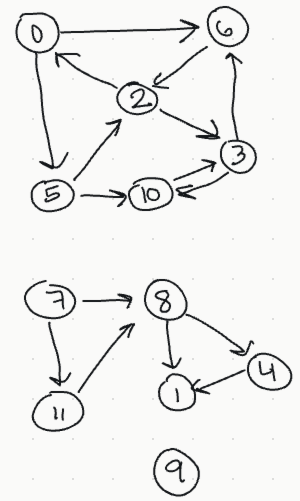
\includegraphics[width=0.2\textwidth]{exercise-02-tinyGex2-graph}
			\caption{Digraph formed by using the input stream constructor to \texttt{Digraph}
			with \texttt{tinyGex2.txt}.}
			\label{fig:tinyGex2}
		\end{figure}
	\end{ex}
	\begin{sol}
		See Figure~\ref{fig:ex-02}.
		\begin{figure}
			\centering
			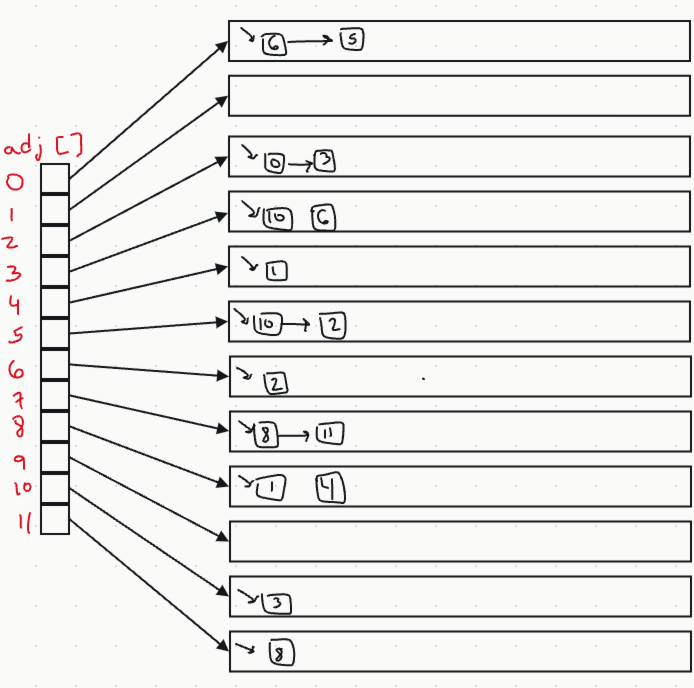
\includegraphics[width=0.6\textwidth]{exercise-02-adjacency-list}
			\caption{Adjacency list for \texttt{Digraph} built from \texttt{tinyGex2.txt}.}
			\label{fig:ex-02}
		\end{figure}
	\end{sol}
	\begin{ex}{3}
		Create a copy constructor for \texttt{Digraph} that takes as input a digraph
		\texttt{G} and creates and initializes a copy of the digraph. Any changes
		a client makes to \texttt{G} should not affect the newly created digraph.
	\end{ex}
	\begin{sol}
		See \texttt{com.segarciat.algs4.ch4.sec2.ex03}.
	\end{sol}
	\begin{ex}{4}
		Add a method \texttt{hasEdge()} to \texttt{Digraph} which takes two \texttt{int}
		arguments \texttt{v} and \texttt{w} and returns \texttt{true} if the graph has
		an edge \texttt{v->w}, \texttt{false} otherwise.
	\end{ex}
	\begin{sol}
		See \texttt{com.segarciat.algs4.ch4.sec2.ex04}.
	\end{sol}
	\begin{ex}{5}
		Modify \texttt{Digraph} to disallow parallel edges and self-loops.
	\end{ex}
	\begin{sol}
		See \texttt{com.segarciat.algs4.ch4.sec2.ex05}.
	\end{sol}
	\begin{ex}{6}
		Develop a test client for \texttt{Digraph}.
	\end{ex}
	\begin{sol}
		See \texttt{com.segarciat.algs4.ch4.sec2.ex06}.
	\end{sol}
	\begin{ex}{7}
		The \emph{indegree} of a vertex in a digraph is the number of directed edges
		that point to that vertex. The \emph{outdegree} of vertex in a digraph is the
		number of directed edges that emanate from that vertex. No vertex is
		reachable from a vertex of outdegree 0, which is called a \emph{sink}; a
		vertex of indegree 0, which is called a \emph{source}, is not reachable from
		any other vertex. A digraph where self-loops are allowed \emph{and} every
		vertex has outdegree 1 is called a \emph{map} (a function from the set of
		integers from $0$ to $V-1$ onto itself). Write a program \texttt{Degrees.java}.
		that implements the following API:
		\begin{lstlisting}[language=java]
		  public class Degrees
	               int Degrees(Digraph G)    // constructor
	               int indegree(int v)       // indegree of v 
	               int outdegree(int v)      // outdegree of v
	Iterable<Integer> sources()              // sources
	Iterable<Integer> sinks()                // sinks
	           boolean isMap()               // is G a map?
		\end{lstlisting}
	\end{ex}
	\begin{sol}
		See \texttt{com.segarciat.algs4.ch4.sec2.ex07}.
	\end{sol}
	\begin{ex}{9}
		Write a method that checks whether a given permutation of a DAG's vertices
		is a topological order of that DAG.
	\end{ex}
		\begin{sol}
		See \texttt{com.segarciat.algs4.ch4.sec2.ex09}.
	\end{sol}
	\begin{ex}{10}
		Given a DAG, does there exist a topological order that cannot result from
		applying a DFS-based algorithm, no matter in what order the vertices adjacent
		to each vertex are chosen? Prove your answer.
	\end{ex}
	\begin{sol}
		No, such a topological order does not exist. It is possible to obtain any
		topological order by using a DFS-based algorithm.
		\begin{proof}
			Let $G$ be a DAG of $V$ vertices, $n=V$, and $\sigma$ be a topological order on $G$.
			If $\sigma_k$ is the $k$th vertex in the order, then $\sigma_n$ must be a sink. Otherwise,
			a vertex would follow it, and we would not have a topological order. If we
			apply DFS to $\sigma_n$, it would return immediately.
			When considering $\sigma_i$, where $i<n$, all vertices that come after $\sigma_i$
			have been marked. Once again, either $\sigma_i$ is a sink (and DFS immediately
			returns), or it points to a vertex that has already been marked. In either case,
			the result is that the vertex is done being processed. We continue this way
			until reaching $i=1$, at which point our DFS-based algorithm ends. Along the way,
			vertices were done in reverse order of $\sigma$, and hence the algorithm
			computes the topological order to be the reverse order of the reverse order
			of $\sigma$, which of course is $\sigma$ itself.
		\end{proof}
	\end{sol}
	
	\begin{ex}{11}
		Describe a family of sparse digraphs whose number of directed cycles grows
		exponentially in the number of vertices.
	\end{ex}
	\begin{sol}
		Digraphs with a center vertex. For example, consider a graph $G$ of $n+1$
		vertices, where for each \texttt{k} there is an edge \texttt{k->0}
		and an edge \texttt{0->k}, where $1\leq k\leq n$. Also, for $k$ and
		$k+1$, there is a pair of edges \texttt{k->(k+1)} and \texttt{(k+1)->k},
		for $k>1$, and for $k=n$, we have \texttt{k->1} and \texttt{1->k}.
		Then $0$ is the center vertex of such a graph. Such a graph is sparse
		because there are $6\cdot n$ edges when there are $n+1$ vertices.
		
		Such a graph is strongly connected. Given subset of the vertices that contains
		$0$, we can create a directed cycle containing $0$. If $S_0$ is the set of
		vertices without $0$, and $\mathcal{P}(S_0)$ is the power set of $S_0$,
		$|\mathcal{P}(S_0)|=2^n$. By appending $0$ to each set, we have at least
		one unique cycle for each set in $\mathcal{P}(S_0)$, meaning at least $2^n$
		cycles.
	\end{sol}
	\begin{ex}{12}
		Prove that the strong components in $G^R$ are the same as in $G$.
	\end{ex}
	\begin{sol}
		\begin{proof}
			Suppose that $C$ is a strong component of $G$, and let $u,v\in C$.
			Then there is a path $p_{uv}$ from $u$ to $v$ and there is a path $p_{vu}$
			from $v$ to $u$. In $G^R$, edges change direction, so the edges in
			the path $p_{uv}$ and reverse to become path $p_{uv}^R$, which is
			now a path from $v$ to $u$. Similarly, $p_{vu}^R$ is a path from $u$
			to $v$. Hence, $u$ and $v$ belong to the same strong component in $G^R$.
			Thus, if $C^R$ is the strong component in $G^R$ that $u$ and $v$ belong
			to, we see that $C\subseteq C^R$.
			
			Now suppose that $w\notin C$, but $w$ belongs to the same component
			as $u$ and $v$ in $G^R$ (that is, $u,v,w\in C^R$). Then, without loss of
			generality, there is a path
			$p_{vw}^R$ from $v$ to $w$ and a path $p_{wv}^R$ from $w$ to $v$ in $G^R$.
			If we reverse the edges of $G^R$ to obtain $(G^R)^R=G$, then the edges
			in both paths are reversed, and we obtain a path $(p_{vw}^R)^R$, from $w$
			to $v$ and a path $(p_{wv}^R)^R$ from $v$ to $w$ in $G$. This implies that
			$w$ and $v$ are in the same strong component, which contradicts the definition
			of $w$. Hence, $w\notin C^R$.
			
			We've just argued that if $w\notin C$, then $w\notin C^R$, which implies that
			$C^R\subseteq C$. We conclude $C=C^R$.
		\end{proof}
	\end{sol}
	\begin{ex}{13}
		Prove that two vertices in a digraph $G$ are in the same strong component
		if and only if there is a directed cycle (not necessarily simple) containing
		them both.
	\end{ex}
	\begin{sol}
		\begin{proof}
			Let $v,w\in G$.
			
			Suppose that $v$ and $w$ belong to the same strong component. Then $w$
			is reachable from $v$ through a directed path $p_{vw}$ and $v$ is reachable
			from $w$ through a directed path $p_{wv}$. By concatenating the paths, we
			create a cycle that contains both $v$ and $w$.
			
			Now suppose that there is a cycle $u_1,u_2,\ldots,u_n,u_1$ containing
			$v$ an $w$. Suppose $v=u_i$ and $w=u_j$, where $j>i$. Then there is a path
			$v_iv_{i+1}\cdots v_{j-1}v_j$ from $v_i$ to $v_j$ and a path
			$v_jv_{j+1}\cdots v_nv_1\cdot v_i$ from $v_j$ to $v_i$. Hence,
			$v$ and $w$ are strongly connected.
		\end{proof}
	\end{sol}
	
	\pagebreak
	\printbibliography
\end{document}